\title{Advanced molecular dynamics modeling}
\author{
        Andreas V. Solbr\aa \\
                University of Oslo\\
		 Department of Computational Physics
}

\documentclass[12pt]{article}
\usepackage{amsmath}
\usepackage{fullpage}
\usepackage{amsthm}
\usepackage{amsfonts}
\usepackage{graphicx}
\usepackage[english]{babel}
\usepackage[T1]{fontenc}
\usepackage{subfigure}
\usepackage{epstopdf}
\epstopdfsetup{update}
\usepackage[hyphens]{url}
\usepackage{gensymb}
\usepackage{verbatim}
%\usepackage{slashed}
\usepackage{amssymb}
\usepackage{amsfonts}
%\usepackage{caption}
%\usepackage{subcaption}
\newtheorem{thm}{Theorem}

%% Define a new 'leo' style for the package that will use a smaller font.
\makeatletter
\def\url@leostyle{%
  \@ifundefined{selectfont}{\def\UrlFont{\sf}}{\def\UrlFont{\small\ttfamily}}}
\makeatother
%% Now actually use the newly defined style.
\urlstyle{leo}


%\usepackage[utf8]{inputenc}
%\usepackage{textcomp}
%\usepackage[T1]{fontenc}




\newcommand{\Fig}[1]{Figure~\ref{#1}}
\newcommand{\fig}[1]{figure~\ref{#1}}
\newcommand{\eq}[1]{equation~\ref{#1}}
\newcommand{\Eq}[1]{Equation~\ref{#1}}

% Shortcuts for including equations
\newcommand{\beq}{\begin{equation}}
\newcommand{\eeq}{\end{equation}}
\def\ivec{\textbf{i}}
\def\jvec{\textbf{j}}
\def\kvec{\textbf{k}}
\def\uvec{\textbf{u}}
\def\vvec{\textbf{v}}
\def\xvec{\textbf{x}}
\def\rvec{\textbf{r}}
\def\Rvec{\textbf{R}}
\def\Fvec{\textbf{F}}
\def\S{\hat{S}}
\def\Svec{\hat{\textbf{S}}}
\def\H{\hat{H}}
\def\ro{\hat{\rho}}
\def\trace{\operatorname{Tr}}
\def\Lop{\hat{L}}
\def\etavec{\hat{\boldsymbol\eta}}
\def\X{\hat{X}}
\def\Y{\hat{Y}}
\def\etaop{\hat{\eta}}
\def\A{\hat{\textbf{A}}}
\def\B{\textbf{B}}
\def\aop{\hat{a}}
\def\aopd{\hat{a}^\dagger}
\def\bop{\hat{b}}
\def\bopd{\hat{b}^\dagger}




% Document formatting
\setlength{\parindent}{0mm}
\setlength{\parskip}{1.5mm}

% Hyper refs
\usepackage[pdftex,colorlinks,breaklinks]{hyperref}
\usepackage{listings}
\usepackage{color}
\usepackage{textcomp}
\definecolor{listinggray}{gray}{0.9}
\definecolor{lbcolor}{rgb}{0.9,0.9,0.9}
\definecolor{pink}{RGB}{255, 119, 255}
\lstset{
	backgroundcolor=\color{lbcolor},
	tabsize=4,
	rulecolor=,
	language=c++,
        basicstyle=\scriptsize,
        upquote=true,
        aboveskip={1.5\baselineskip},
        columns=fixed,
        showstringspaces=false,
        extendedchars=true,
        breaklines=true,
        prebreak = \raisebox{0ex}[0ex][0ex]{\ensuremath{\hookleftarrow}},
        frame=single,
        showtabs=false,
        showspaces=false,
        showstringspaces=false,
        identifierstyle=\ttfamily,
        keywordstyle=\color[rgb]{0,0,1},
        commentstyle=\color[rgb]{0.133,0.545,0.133},
        stringstyle=\color[rgb]{0.627,0.126,0.941},
	title=\lstname
}

\newcounter{subproject}
\renewcommand{\thesubproject}{\alph{subproject}}
\newenvironment{subproj}{
\begin{description}
\item[\refstepcounter{subproject}(\thesubproject)]
}{\end{description}}
\date{\today}

\begin{document}
 \maketitle
 \begin{abstract}
The goal of this project is to gain experience in more advanced modeling in molecular dynamics. It will build directly on the previous project. 
 \end{abstract}
 In the previous project we made a simple model for an Argon gas. In this project, we are interested in using and expanding on our model to look at some more interesting system. We want to create much larger systems than earlier, and the first thing we should do is to optimize and parallelize our code
 \section{Optimization}
 \subsection{Parallelization using OpenMP}
 OpenMP is a wonderful ``plug and play'' parallelization API for situations where all your parallel threads share memory. Say you want have a loop that sums the first $N$ terms in the harmonic series. In order to parallelize this, all you need to do is to go from
 \begin{lstlisting}[language=c++]
double sum = 0;

for(n=1;n<=N;n++){
  sum += 1./n;
  }
 \end{lstlisting}
 to
  \begin{lstlisting}[language=c++]
double sum = 0;
#pragma omp parallel{
  double loc_sum = 0;
  #pragma omp for
  for(int n=1;n<=N;n++){
    loc_sum += 1./n;
  }
  #pragma omp critical{
    sum += loc_sum;
  } 
}
 \end{lstlisting}
 The variable \verb loc_sum  is created privately for each thread as it is inside the parallel scope defined by the first pragma statement. The critical statement ensures that the different threads write to the global variable \verb sum  one at a time. If we know that one part of our code stands out as particularly time-consuming, it is often well worth while to try to parallelize it using openMP at first, as the implementation is so simple. In our case, the time-consuming part is the calculation of the forces, as this loops over many different particle pairs. We can test our code for different numbers of particles and processors. The result is shown i figure \ref{fig:1}. We see a clear improvement when going from 1 to 2 processors, but after this there is almost no speedup. For smaller systems the computation time even increases! This is most likely due to overhead from adding the forces matrices together. 
 
 \begin{figure}
  \centering
  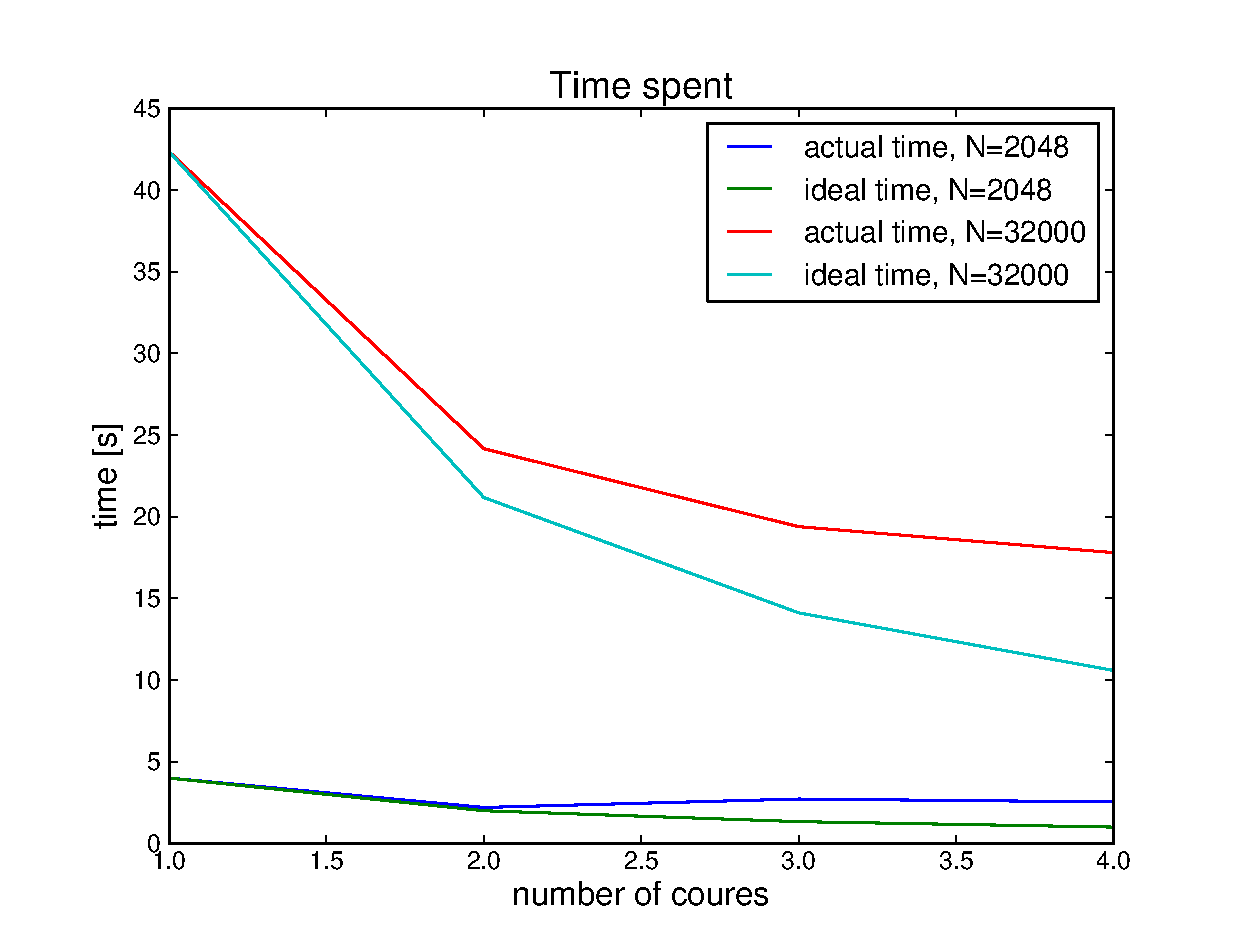
\includegraphics[width=10cm]{parallel.eps}
\caption{\label{fig:1} The figure shows the time spent for $N=2048$ and $N=32000$ particles as a function of cpu cores when using openMP, for a test simulation of 100 time steps.}
 \end{figure} 

 \subsection{Optimizing the code for efficiency}
 We should note that we can also gain a lot from just writting our code in a more optimized way. In the previous project we used vectors and matrices from the armadillo c++ library. This has the advantage of producing cleaner code, but it comes at the price of efficiency. The most important point is to stay away from armadillo functions such as \verb dot  and \verb norm . These are terribly inefficient, and will often take up to 10 times as much time as a hardcoded version. Furthermore, armadillo vectors have overloaded +/- operators, that are quite slow compared to writing the additions out element by element. Using these changes gave an overall speedup factor of around 10, and was absolutely essential in order to make the code usable for large scale experiments.
 
 \section{Generating a nanoporous material}
 We will now look into ways of generating nanoporous matrial. As the c++ code can continue a simulation from an .xyz-file, we can thermalize our system in one simulation, do any manipulation in Python for simplicity and continue the simulation from our manipulated .xyz-file. Including the possibility of starting from a given .xyz-file in our program is very usefull, as it gives us an easy way to change parameters in the experiment such as thermostats and, as in this case, freeze some of the particles. 
 
 As a simple test, we can thermalize a system of liquid Argon in a $20\times20\times 20$ cell with cell size $b = 5.72$ Å at $T = 0.851$, cut out a cylinder of 2 nm, and freeze all the particles outside this cylinder. The result of such an experiment is shown in figure \ref{fig:2}
 
  \begin{figure}
  \centering
  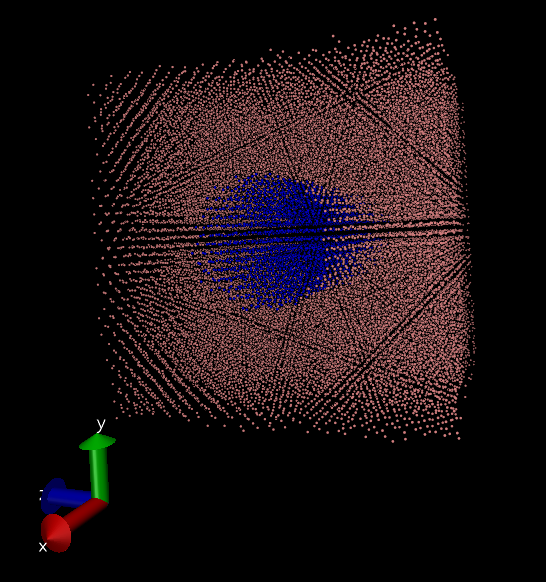
\includegraphics[width=10cm]{cylinder.png}
\caption{\label{fig:2} The figure shows a system with a cylinder of size 2 nm}
 \end{figure} 
 
 \subsection{Model for nanopourous material}
 There are several different ways of generating a nanoporous material. One can for instance slowly expand the size of the size of our system while cooling it. Here we will look at a much simpler method. We simply make a a collection of spheres with radii in the range 2-3 nm, and freeze either the particles inside the spheres, or the particles outside. For our system, we will make 20 spheres and freeze the paricles outside the spheres. It is useful to find the porosity of such a system, that is, the relative amount of pore space in the volume. An easy way to do this is to assume that each particle takes up the same amount of space, and simply count the particles which are not frozen by this procedure. Since we allow the spheres to overlap, and be partially outside the system, it will be troublesome to find an analytic expression for this ratio, and we rather find it numerically through several experiments the results of these experiments are shown i figure \ref{fig:3}, and gives an average porosity around 63\%
. We note that each sphere has an average volume of $4\pi/3 \langle r^3 \rangle \approx 68 \rm{nm}^2$ so that 20 non-overlapping spheres all inside the box of sides $20 \times 5.72$nm would yield an average porosity of 91\%.
 
   \begin{figure}
  \centering
  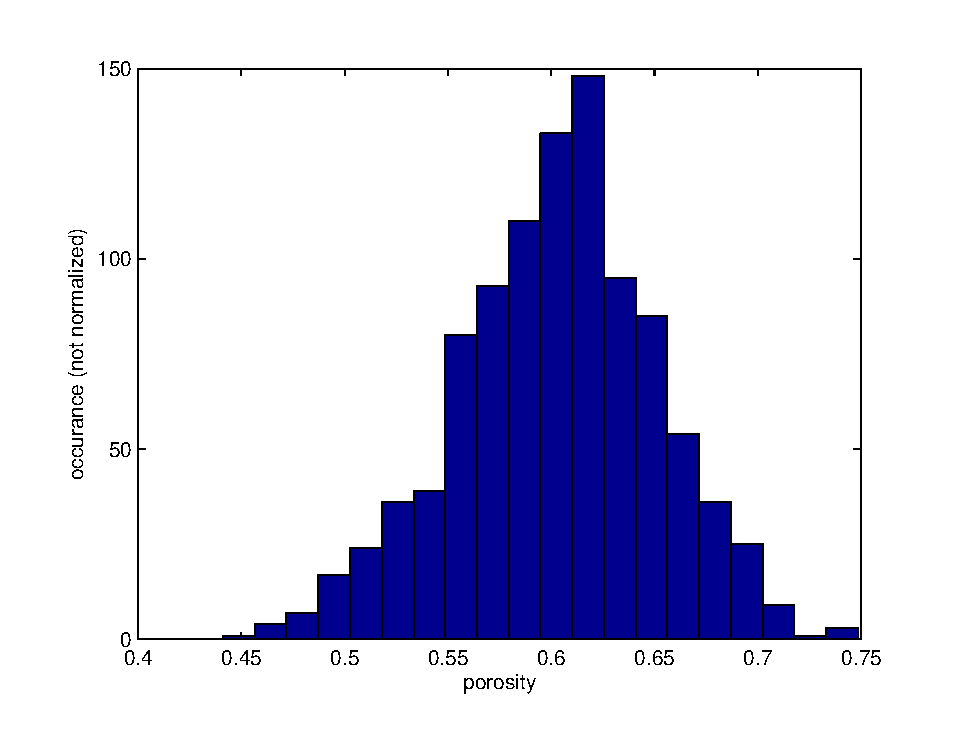
\includegraphics[width=12cm]{porosity.eps}
\caption{\label{fig:3} The figure shows the porosity distribution of a system of 20 spheres.}
 \end{figure} 
 
 We can now visualize our system. Figure \ref{fig:4} shows the result of such and experiment, where the system has been thermalized at $T = 1.05$ after the particles outside the spheres.
 
    \begin{figure}
  \centering
  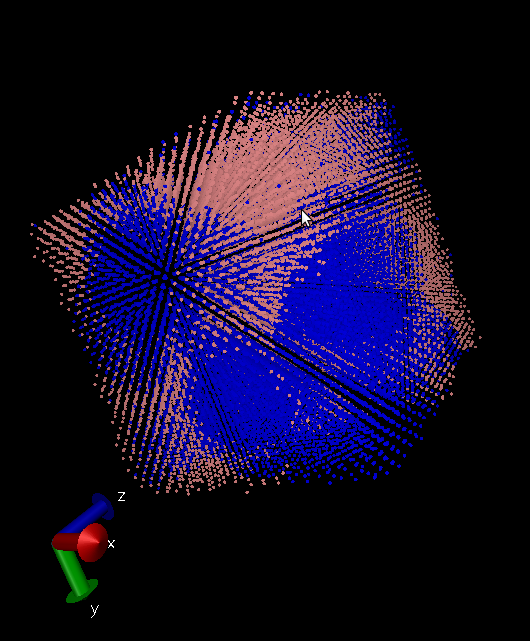
\includegraphics[width=12cm]{nanopores.png}
\caption{\label{fig:4} The figure shows a nanoporous material, created as discussed in the text.}
 \end{figure} 
 
 \subsection{Low-density fluid in a nanoporous material}
 We now want to model the flow a low density through the fluid we have created. This is a task well suited for our Python framework. We simply loop over all the unfrozen atoms and set a 50\% chance of deleting them. This can be found in the python function \verb removeSomeUnFrozenAtoms(self,eps) . We can messure the pressure of the system, as well as the pressure distribution in space. One way to do the latter is to calculate the pressure for each cell, and then plot these somehow. In figure \ref{fig:5}, they have been plotted in ovito coloring the cell dots by amount of pressure
 
   \begin{figure}
  \centering
  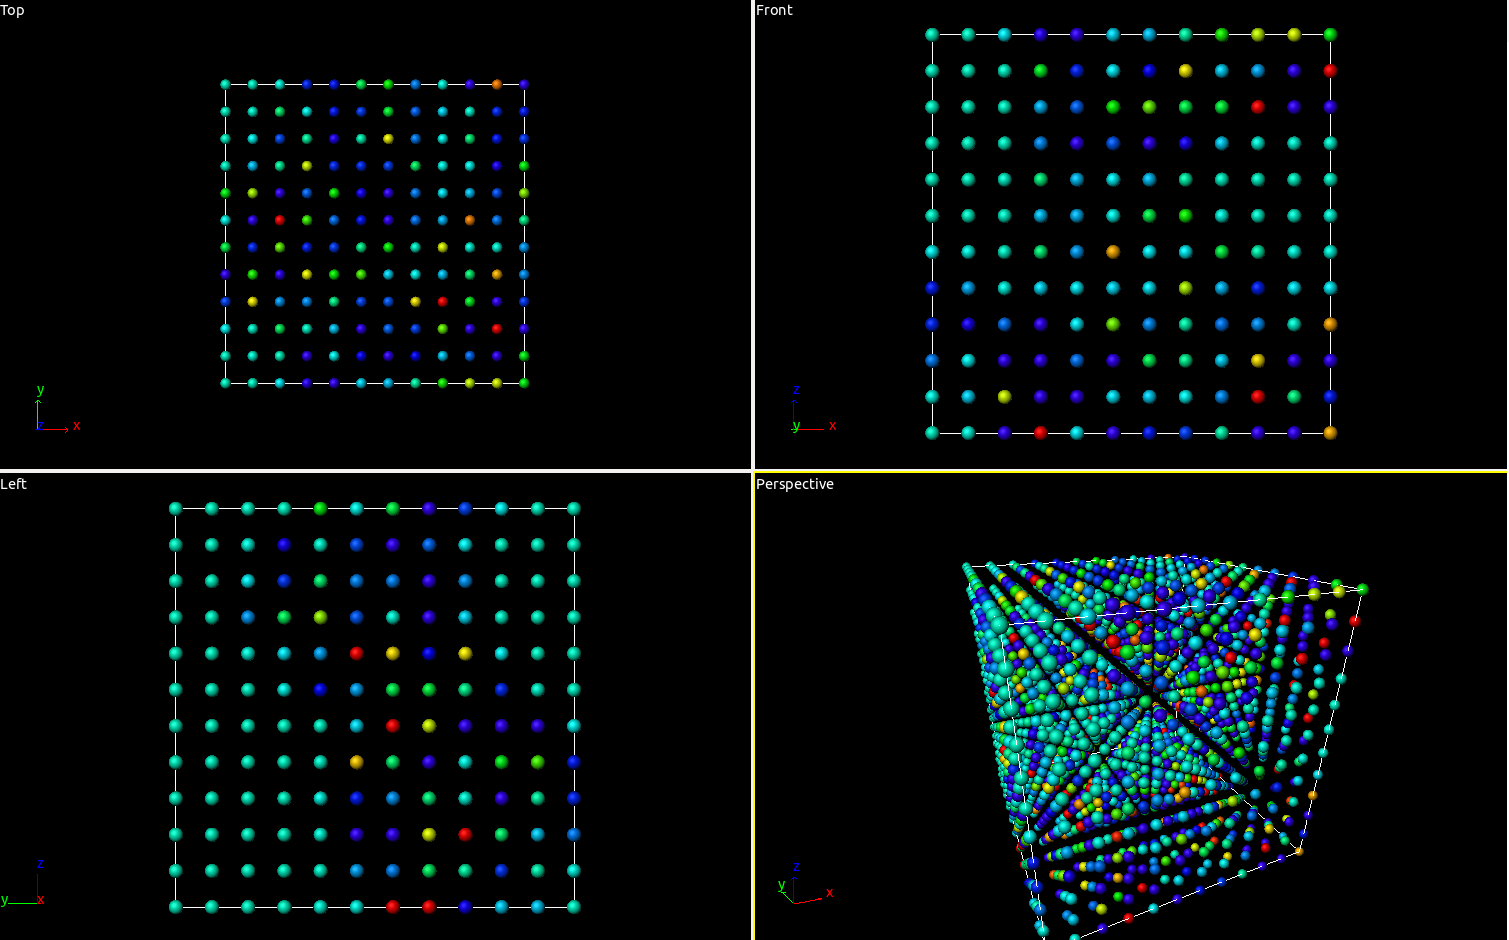
\includegraphics[width=18cm]{pressure.png}
\caption{\label{fig:5} The figure the pressure distribtion of the system. The pressures are in the range -50 to 100 [MD units], with red denoting the highest pressures.}
 \end{figure} 
 
    \begin{figure}
  \centering
  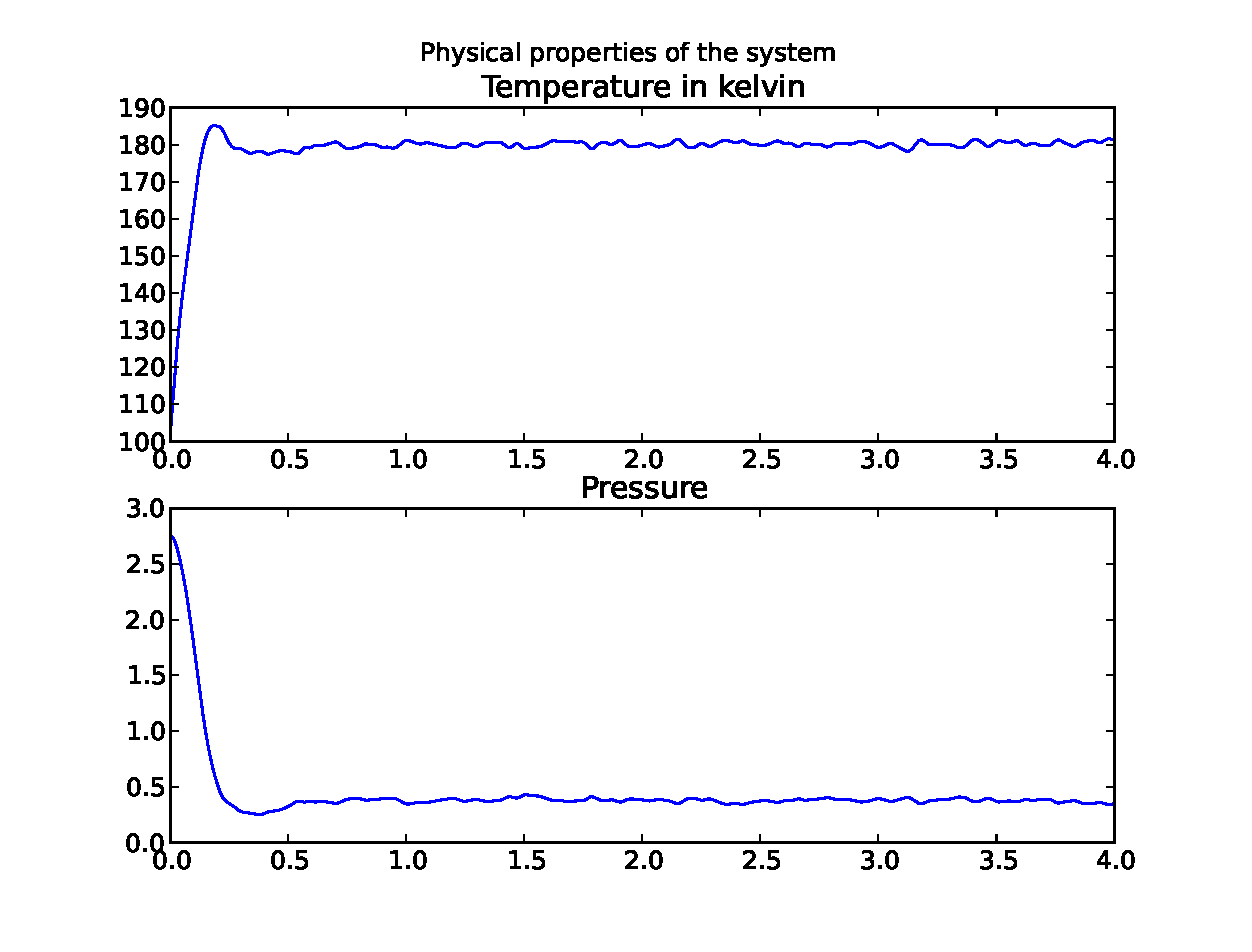
\includegraphics[width=18cm]{pressuretime.eps}
\caption{\label{fig:7} The figure shows the pressure of the low density fluid as a function of time. Both pressure and time are in MD units.}
 \end{figure} 
 
 \section{Diffusion in a nanopourous material}
 Figure \ref{fig:6} shows the average square displacement of the low-density fluid.
 
  \begin{figure}
  \centering
  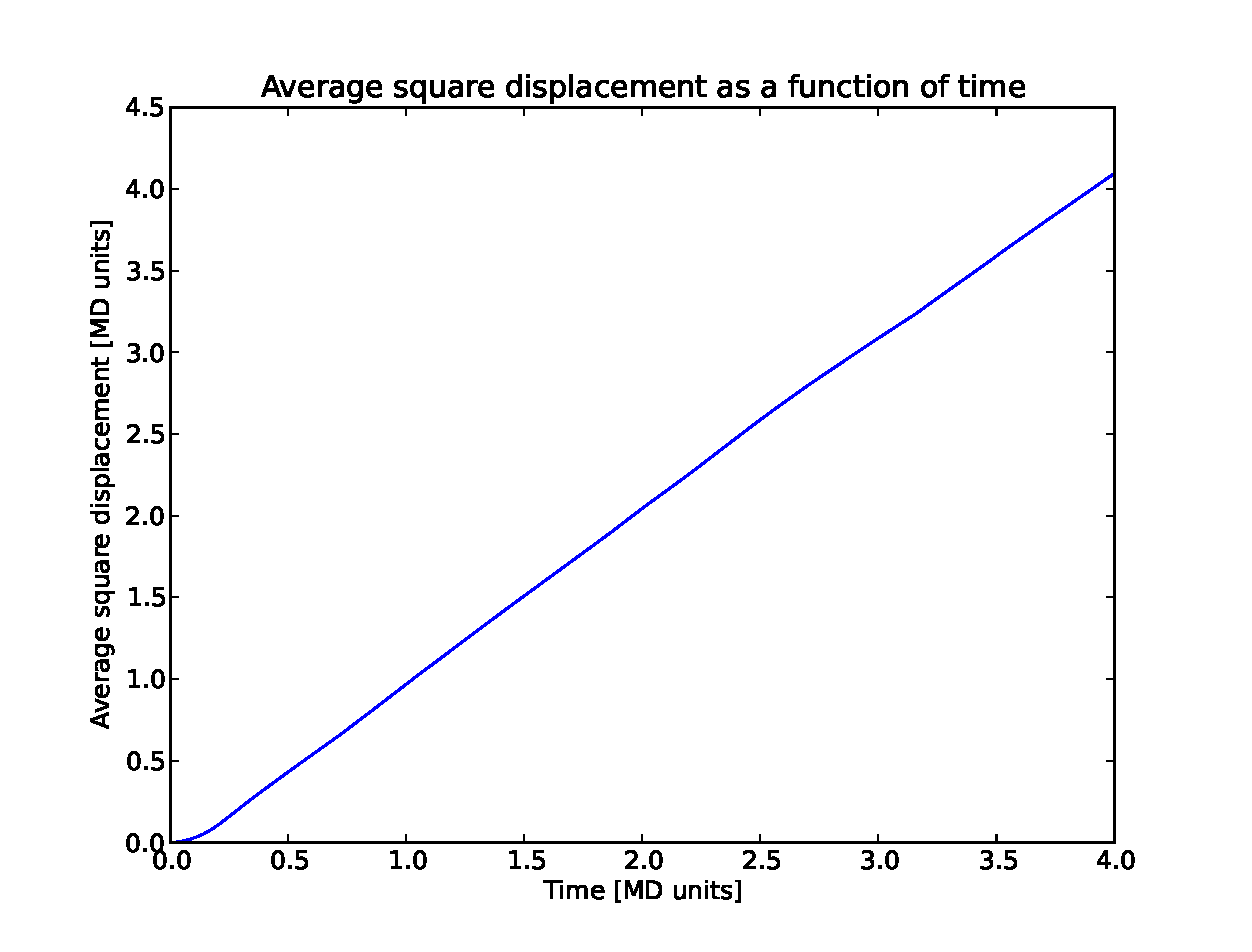
\includegraphics[width=10cm]{avgsqdis.eps}
\caption{\label{fig:6} The figure shows the average square displacement of the low-density fluid when thermalized at $T = 1.5$.}
 \end{figure} 
 
 
 \section{Flow through a nanoporous material}
 We can induce a flow in the material by introducing an external force, $\textbf{F} = F_x \ivec$ acting on each atom - similar to gravity. In the case of flow in a gravitational field, Darcy's law is usually formulated as 
 \begin{equation}
  U = {k\over \mu}(\nabla P - \rho g) 
 \end{equation}
 For a system like flow thorugh a cylinder, we can ignore the $\nabla P$-term and note that $\rho g = Nmg/V = n F$, where $n=N/V$ is the number density of particles and $F = mg$ is the force exerted by the gravitational potential.
 
It is interesting to measure the flow profile of our liquid and cylinder system. From continuum models, the flow profile should be $u(r) \propto a^2-r^2$ where $a$ is the radius of the cylinder, and the density profile should be constant. Figure \ref{fig:8} shows these properties for a normal density fluid, while \ref{fig:9} show these for a low density fluid, where we have set $F = 1.0 \epsilon/\sigma$. The results seem to be in good agreement with the theory, with the note that for high density liquids, there will be some structure in the density due to the particle interactions. We can use these results to measure the viscosity of the fluid, as for a cylindrical pipe, the velocity profile can be shown to be 
\begin{equation}
 u(r) = {\Delta P \over L} {1 \over 4\mu }(a^2 - r^2)
\end{equation}
where $\Delta P$ is the pressure difference in the pipe, $L$ is the length of the pipe, $\mu$ is the viscosity of the fluid, $a$ is the radius of the pipe and $r$ is the distance from the radius. Using $u(0) = 2.5\sigma/\tau$ for the high density fluid and $u(0) = 3.5\sigma/\tau$ for the low density fluid, and in our MD units, $a = 5.9\sigma$. The pressure difference is simply $\Delta P = \rho g \Delta h = nFL = NFL/V$ inside the cylinder where $N$ is the total number of particles, $V$ is the volume of the cyllinder. The number density is $n=0.84\sigma^{-3}$ for the high density and $n=0.42\sigma^{-3}$ for the low density.
\begin{equation}
 \mu = {nFa^2\over 4u(0)}
\end{equation}
which gives $\mu = 11.7 {m\over \sigma \tau}$ for the high density fluid and $\mu = 5.8 {m\over \sigma \tau}$ for the low density fluid, where $m$ is the mass of the Argon atom (i.e. our unit of mass).


\begin{figure}[ht]
\centering
\subfigure[velocity distribution]{
	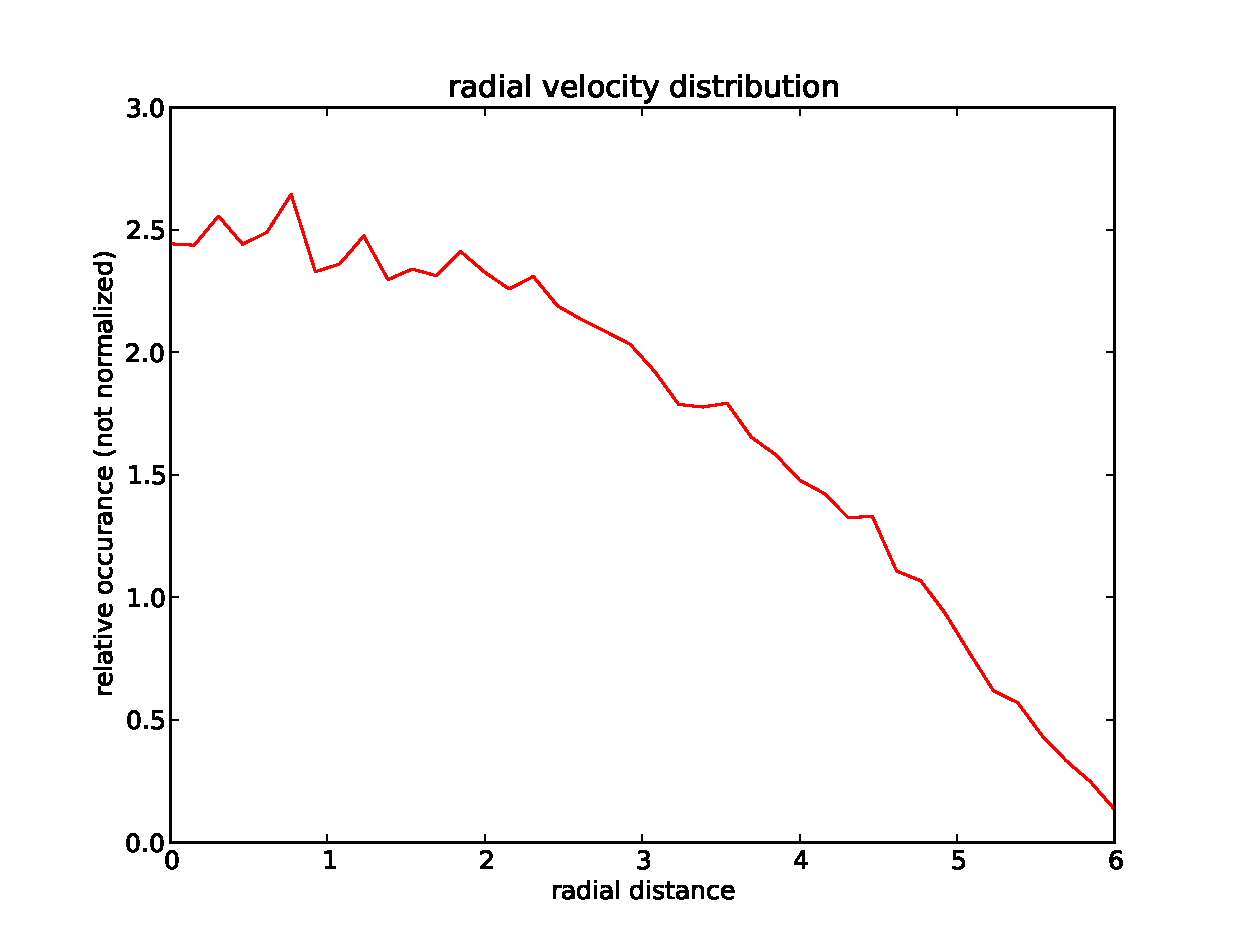
\includegraphics[width=7cm]{densevel.eps}
	\label{fig:subfig1}
}
\subfigure[density distribution]{
	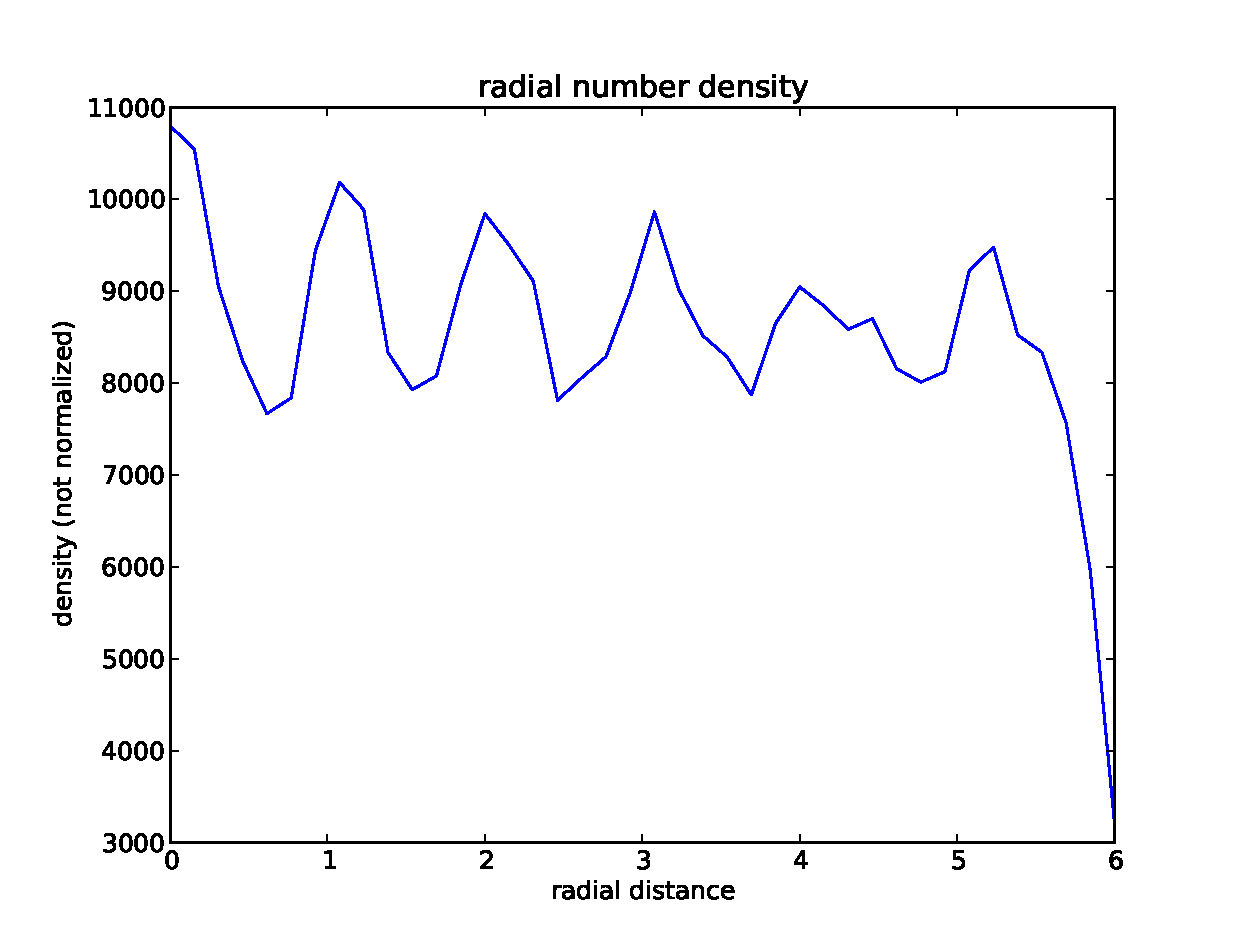
\includegraphics[width=7cm]{densedens.eps}
	\label{fig:subfig2}
}
\caption[Optional caption for list of figures]{The plots show the distribution of the velocity and the distribution of particles in a cylinder filled with a dense liquid subject to a constant force at 500 K.}
\label{fig:8}
\end{figure}
 
 \begin{figure}[ht]
\centering
\subfigure[velocity distribution]{
	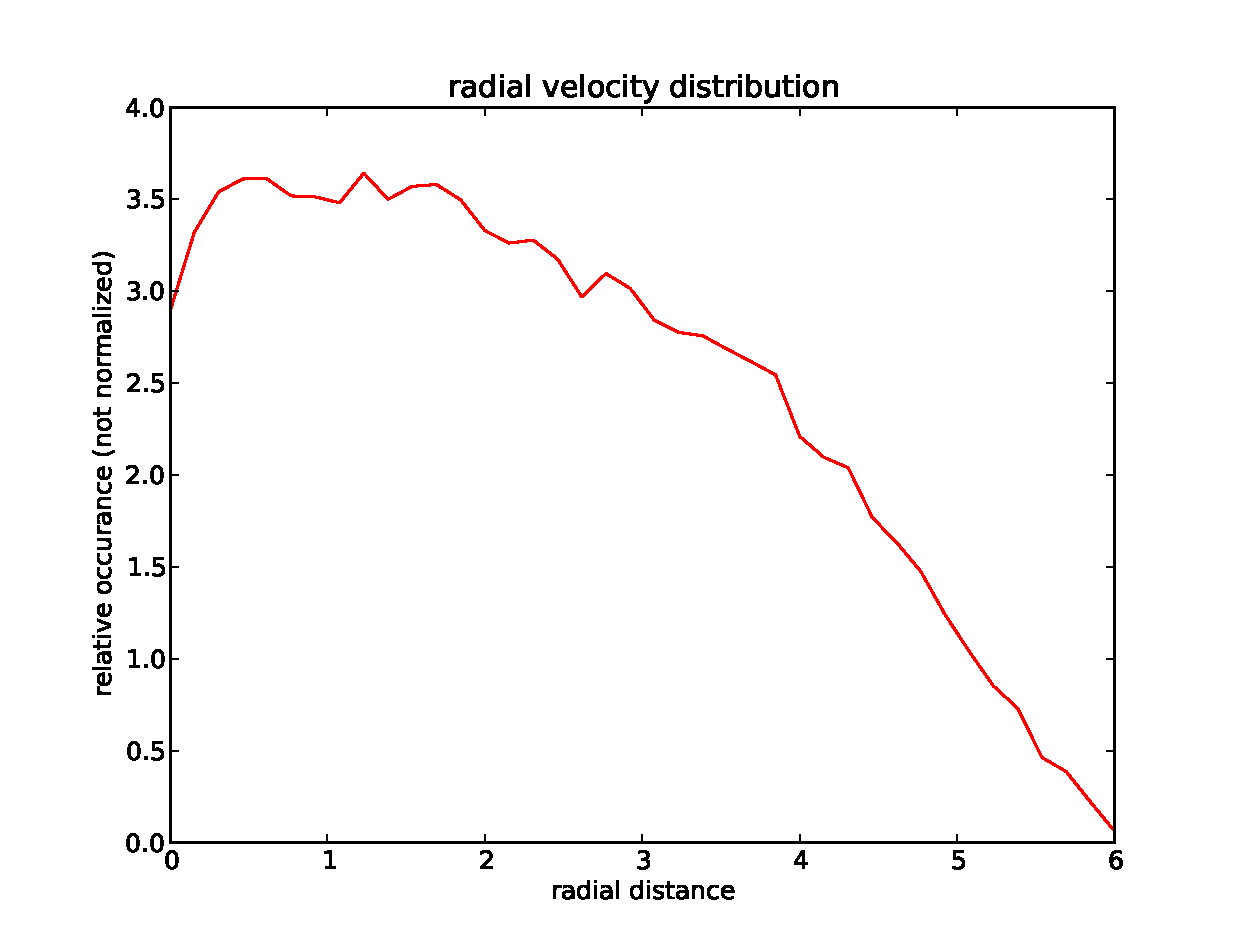
\includegraphics[width=7cm]{lowdensevel.eps}
	\label{fig:subfig3}
}
\subfigure[density distribution]{
	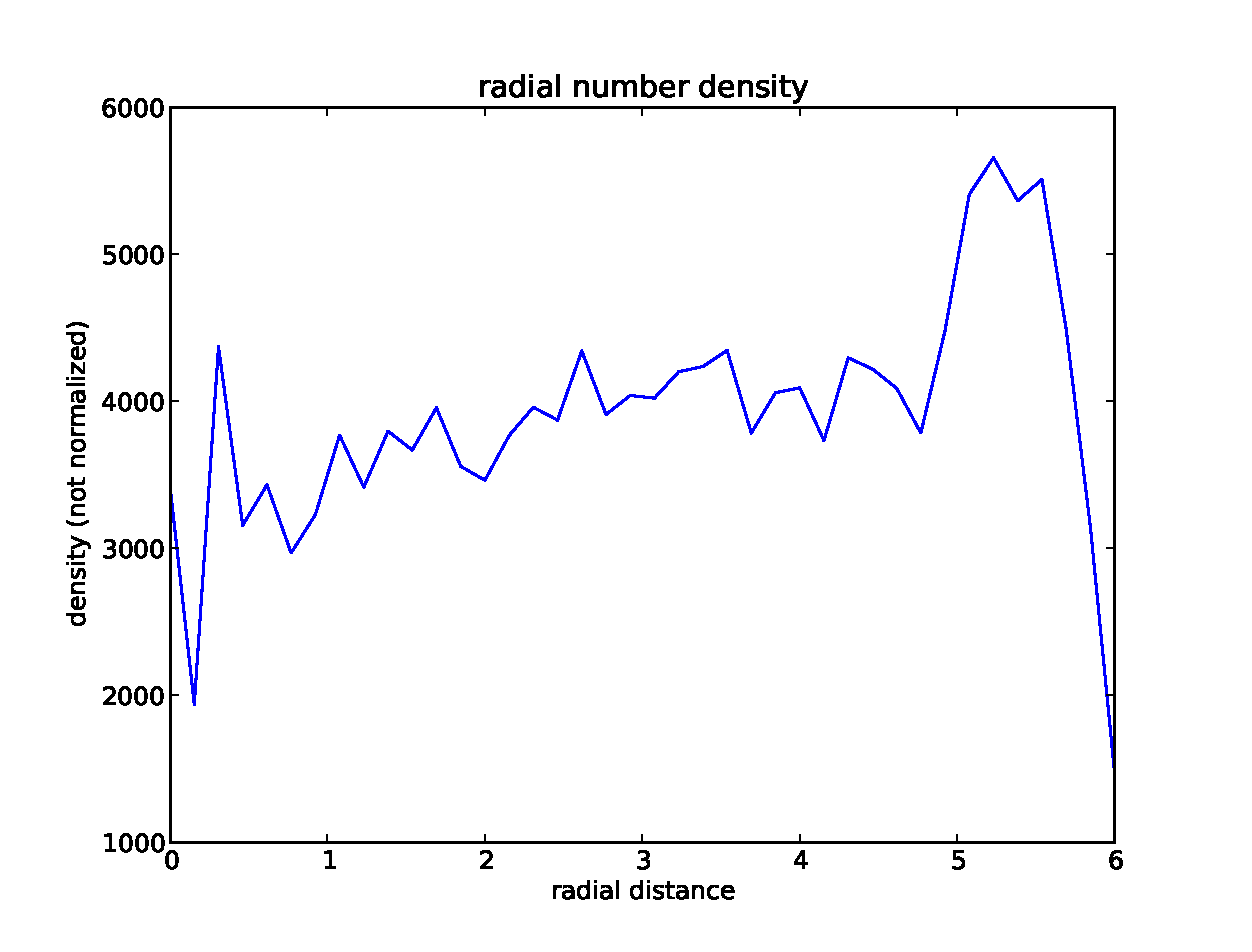
\includegraphics[width=7cm]{lowdensedens.eps}
	\label{fig:subfig4}
}
\caption[Optional caption for list of figures]{The plots show the distribution of the velocity and the distribution of particles in a cylinder filled with a low-density liquid subject to a constant force at 500 K.}
\label{fig:9}
\end{figure}

\section{Permeability}
Finally, we will investigate the permeability of our nanoporous materials with varying porosities. To do this. we simply generate a large collection of systems to simulate with different porosities. We can find the permeability from Darcy's law; 
\begin{equation}
 Q = {kA \over \mu}{\Delta P \over L}. 
\end{equation}
The results of many experiments is shown in figure \ref{fig:10}.
  \begin{figure}
  \centering
  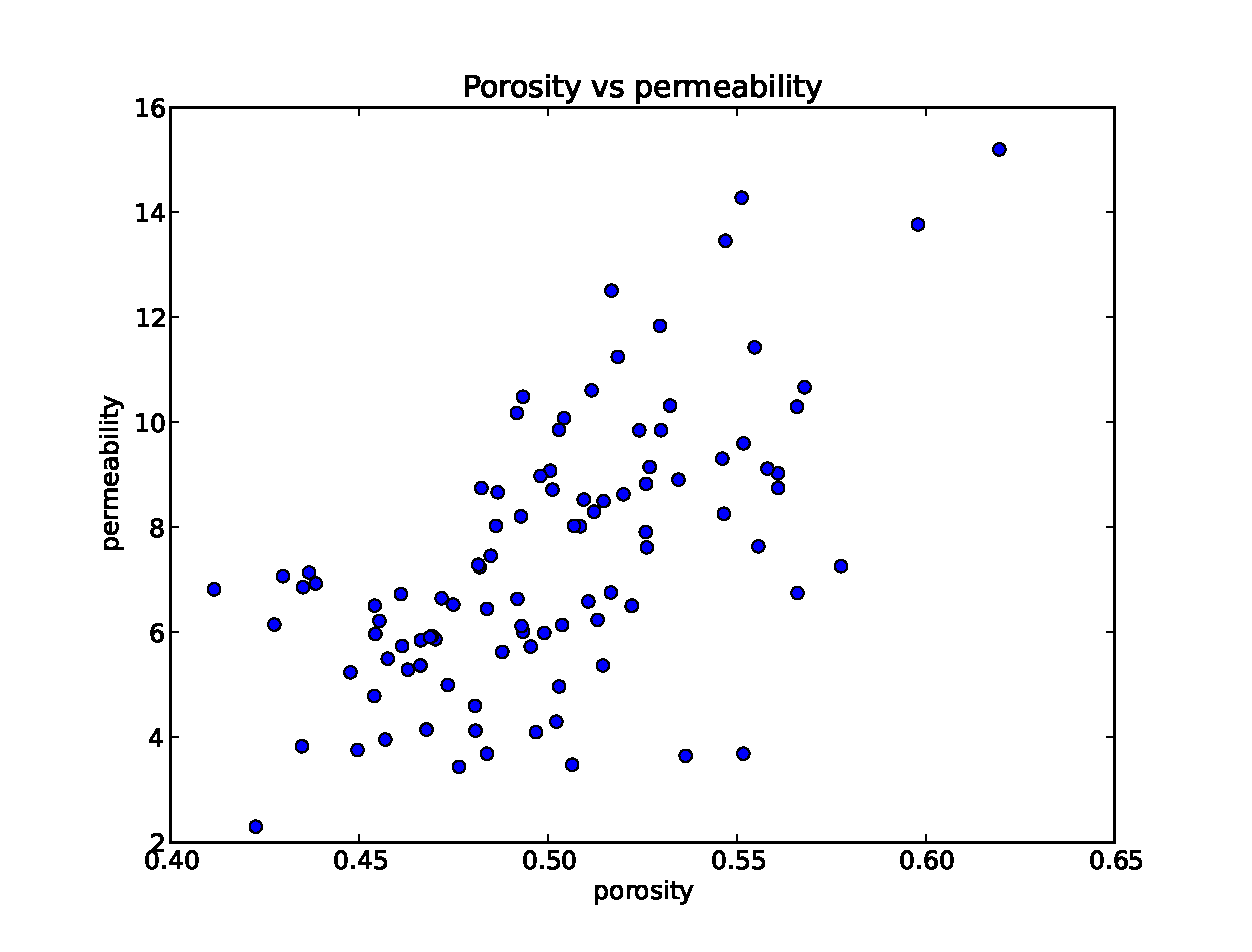
\includegraphics[width=10cm]{perm.eps}
\caption{\label{fig:10} Permeability and porosity}
 \end{figure} 

 \end{document}